% Theorie: Physikalische Grundlagen von Versuch/Messverfahren, Gleichungen ohne Herleitung knapp erklären
\section{Theorie}
\label{sec:theorie}

Als Grundlage des Versuches dient die elektromagnetische Wellentheorie, wobei die Ausbreitung von Licht 
mit Hilfe der Maxwellschen Gleichungen 
\begin{align}
    \nabla \times \vec{H}&=\vec{j}+\varepsilon \varepsilon_{0} \partial_t \vec{E} \quad \text{und} \\
    \nabla \times \vec{E}&=-\mu \mu_{0} \partial_t \vec{H}
    \label{eqn:maxwell}
\end{align}
beschrieben wird.
Im folgenden werden nicht-ferromagnetische und nicht elektrisch leitende Materialien betrachtet, somit gilt $\mu \approx 1$
und $\vec{j} =0$.
Die elektrische und magnetische Arbeit 
\begin{align*}
    W_\text{{elektrisch}} &\coloneq \frac{1}{2} \varepsilon \varepsilon_0 \vec{E}^2 \quad \text{und}\\
    W_{\text{magnetisch}} &\coloneq \frac{1}{2} \mu_0 \vec{H}^2
\end{align*}
stellen den Zusammenhang zwischen Energie pro Volumeneinheit eines elektrischen beziehungsweise magnetischen Feldes dar.
Der Poynting Vektor 
\begin{align}
    \vec{S} &= \vec{E} \times \vec{H} \quad  \text{und}\\
    |\vec{S}| &= v \varepsilon \varepsilon_0 \vec{E}^2
    \label{eqn:poynting}
\end{align}
besitzt die Dimension Leistung/Fläche und stellt die Strahlungsleistung pro Flächeneinheit eines 
elektromagnetischen Feldes dar.
Beim Einfallen einer Welle aus dem Vakuum auf eine Grenzfläche unter einem Winkel $\alpha$, wird ein Bruchteil dieser
refelktiert und der andere dringt in das Medium ein. Der Lichtstrahl, welcher in das Medium eindringt erfährt eine Richtungsänderung 
und wird so gebrochen, dass der Beugungswinkel $\beta < \alpha$ ist. Es werden nur nicht absorbierende Medien verwendet und es gilt somit
\begin{align*}
    \symup{S}_e \symup{F}_e &= \symup{S}_r \symup{F}_e + \symup{S}_d \symup{F}_d \quad \text{oder}\\
    \symup{S}_e \cos \alpha &= \symup{S}_r \cos \alpha + \symup{S}_d \cos \beta .
\end{align*}
Diese Gleichung kann umgeschrieben werden zu 
\begin{equation}
        c \varepsilon_0 \vec{E}_e^2 \cos \alpha=c \varepsilon_0 \vec{E}_r^2 \cos \alpha+v \varepsilon \varepsilon_0 \vec{E}_d^2 \cos \beta.
        \label{eqn:strahlung}
\end{equation}
Für den Brechnungsindex ergibt sich das Verhältnis
\begin{equation}
    n = \frac{c}{v}.
    \label{eqn:brechungsindex}
\end{equation}
Aus den Maxwellschen Gelichungen \eqref{eqn:maxwell} ergibt sich die Maxwellsche Relation
\begin{equation}
    n = \varepsilon^2 .
    \label{eqn:relation}
\end{equation}
Aus der Mexwellschen Relation \eqref{eqn:relation} und der \autoref{eqn:strahlung} ergibt sich 
\begin{equation}
    \left(\vec{E}_e^2-\vec{E}_r^2\right) \cos \alpha=\mathrm{n} \vec{E}_d^2 \cos \beta .
\end{equation}

Die Polarisationsrichtung der einfallenden Welle $\vec{E}_e$ relativ zur Einfallsebene ist entweder senkrecht polarisiert oder parallel polrarisiert,
sodass
\begin{equation}
        \vec{E}_e=\vec{E}_{\perp}+\vec{E}_{\|}
\end{equation}
gegeben ist.
Zunächst wird die Polarisation senkrecht zur Einfallsebene betrachtet. Für den parallel polarisierten Teil  $\vec{E}_{\|}$ geht hervor, dass 
dieser tangential zur Grenzfläche schwingt. In der \autoref{fig:bild1} wird die Reflexion eines Lichtstrathls an einer Grenzfläche 
dargestellt.

\begin{figure}[H]
	\centering
	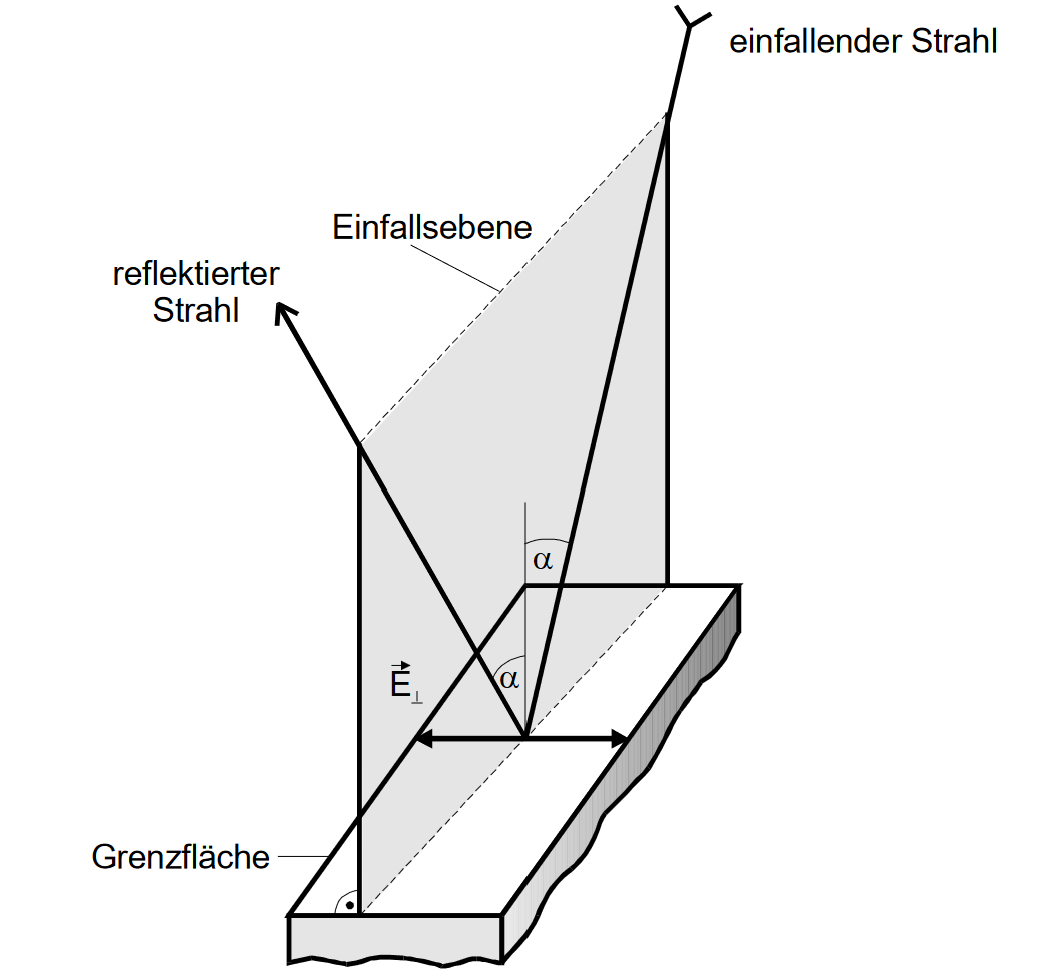
\includegraphics[width=0.5\linewidth]{content/grafik/bild1.png}
	\caption{Darstellung eines reflektierten Lichtstarhls an einer Grenzfläche \cite{fresnel}.}
	\label{fig:bild1}
\end{figure}